\documentclass[a4paper,10pt]{beamer}

\usepackage[utf8]{inputenc}
\usepackage{fontspec}
\usepackage{amsmath}
\usepackage{amssymb}
\usepackage{graphicx}
\usepackage{subcaption}
\usepackage{comment}
\usepackage{wrapfig}
\usepackage{color}

\usefonttheme{professionalfonts}

\usefonttheme[]{structurebold}

\usetheme{Copenhagen}
\usecolortheme{rose}
\usecolortheme{dolphin}
\useinnertheme{circles}
\useoutertheme{tree}

\addtobeamertemplate{navigation symbols}{}{%
	\usebeamerfont{footline}%
	\usebeamercolor[fg]{footline}%
	\hspace{1em}%
	\insertframenumber/\inserttotalframenumber
}


\setmainfont[Path=/usr/share/fonts/truetype/calibri/,
BoldItalicFont=calibriz.ttf,
BoldFont      =calibrib.ttf,
ItalicFont    =calibrii.ttf]{calibri.ttf}

\newcommand{\BS}[1]{\boldsymbol{#1}}
\newcommand{\E}[1]{\mathbb{E}\left[ #1 \right]}
\newcommand{\sqb}[1]{\left[ #1 \right]}

\definecolor{burgundy}{RGB}{128,0,32}
\definecolor{darkgreen}{RGB}{4,110,0}

\title{Generalized Langevin Equation}
\subtitle{Stochastic Differential Equations}
\author{Sankarasubramanian Ragunathan \newline \newline 389851}
\institute{\textbf{RWTH Aachen}}
\date{}


\begin{document}
	\begin{frame}
		\titlepage
		\centering
		
\includegraphics[width=0.2\textwidth]{RWTH_Aachen_University_Logo.eps}
	\end{frame}

	\begin{frame}
		\tableofcontents
	\end{frame}

	\begin{frame}
		\small
		\section{Scope of the Project}
		\frametitle{Scope of the Project}
		
		\begin{itemize}
			\item[What?]{Generalized Langevin Dynamics is a modeling technique that can be used to model anomalous diffusive phenomena observed in viscoelastic fluid flow and in biological systems.}
			
			\item[Why?]{Anomalous diffusion problems: Langevin model fails to capture sub-diffusive and super-diffusive behavior which the GLE succeeds in capturing. But GLE is \textit{Non-Markovian} i.e. \texttt{memory kernel} depends on the history of velocity. This issue is overcome by using Extended Variable GLE that considers a finite dimensional subspace for the \texttt{memory kernel}.}
			
			\begin{figure}[H]
				\centering
				\includegraphics[width=0.35\linewidth]{./Plots/Diffusion.pdf}
				\caption{Anomalous Diffusion: Linear,Sub and Super Diffusive nature}
			\end{figure}
		\end{itemize}
	\end{frame}

	\begin{frame}
	\begin{itemize}
		\item[Where?]{Applications of GLD include but are not restricted to micro-rheology, biological systems, nuclear quantum effects and systems in which anomalous diffusion arise.}
		
		\item[How?]{The theory behind extended variable GLD is studied. Accuracy of Implicit/Explicit Euler and Splitting Numerical schemes are also tested to find out the optimal scheme. Study the sensitivity of the solution to the changes in the parameters of the extended variable Prony series.}
	\end{itemize}
	\end{frame}

	\begin{frame}
		\section{Introduction}
		\frametitle{Introduction}
		
		\quad \textbf{Langevin Dynamics} is a modeling technique in which the motion of a set of massive bodies in the presence of a bath of smaller solvent particles is directly integrated, while the dynamics of the solvent are "averaged out".
		
		\begin{figure}[H]
			\flushleft
			\begin{subfigure}[b]{0.35\linewidth}
				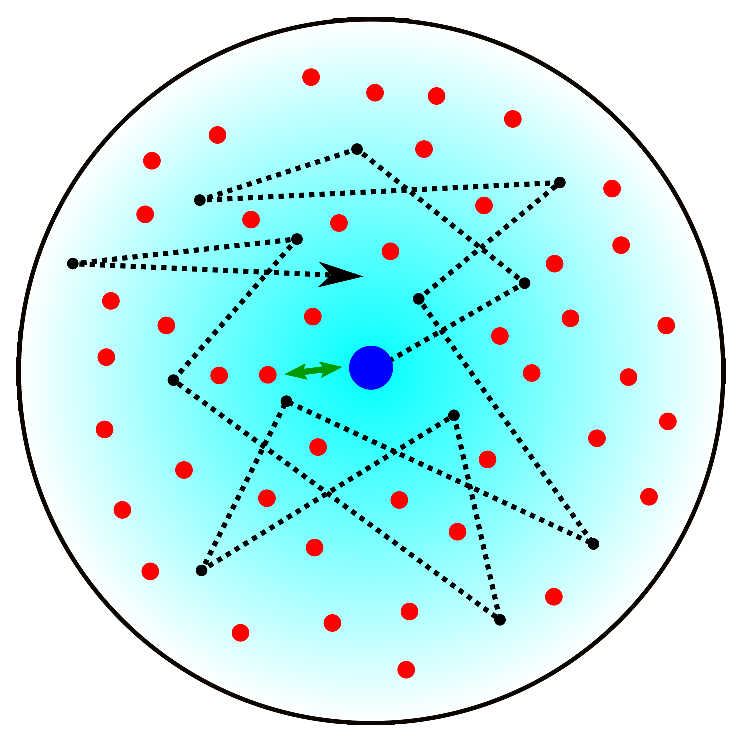
\includegraphics[width=\linewidth]{./Plots/HeatBathAlt.eps}
				\caption{Big particle interacting with the smaller particles.}
				\label{fig:HeatBath}
			\end{subfigure}
			\hfill
			\begin{subfigure}[b]{0.6\linewidth}
				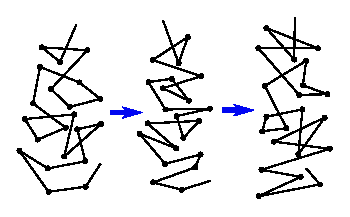
\includegraphics[width=\linewidth]{./Plots/ParticleEvolution.eps}
				\caption{Evolution of a molecule over time due to interaction with smaller particles.}
				\label{fig:ParticleEvolution}
			\end{subfigure}
		\end{figure}
		
	\end{frame}		
	
	\begin{frame}
		%\footnotesize
		\section{Generalized Langevin Equation}
		\frametitle{Generalized Langevin Equation}
		\framesubtitle{Mathematical Model}
		
		GLE equations are based on \textit{Ornstein-Uhlenbeck} equations
	
		\begin{block}{GLE Equations}
			\begin{align}
			d\BS{X}(t) &= \BS{V}(t) dt \\
			\BS{M} d\BS{V}(t) &= \BS{F}^{c}(\BS{X}(t)) dt - \int_{0}^{t} \BS{\Gamma}(t-s) \BS{V}(s) ds dt + \BS{F}^{r}(t)dt \\
			\BS{X}(0) = \BS{X}_{0}, &\qquad \BS{V}(0) = \BS{V}_{0} \qquad (\text{Initial Conditions})
			\end{align}
		\end{block}
	
		\begin{block}{Temporally Non-Local Drag Force ($\BS{F}^{d}$)}
			\begin{align}
			\BS{F}^{d} (t) = - \int_{0}^{t} \BS{\Gamma}(t-s) \BS{V}(s) ds dt
			\end{align}
		\end{block}
	\end{frame}

	\begin{frame}
		\small
		\frametitle{Generalized Langevin Equation}
		\framesubtitle{Mathematical Model}
		\begin{table}[H]
			\begin{tabular}{l l}
				$\BS{F}^{c} : \mathcal{R}^{d N_{p}} \to \mathcal{R}^{d N_{p}}$ & Conservative Force \\
				$\BS{F}^{r} : \mathcal{R}^{d N_{p}} \to \mathcal{R}^{d N_{p}}$ & Random Correlated Force \\
				$\BS{M}$ & Diagonal Mass Matrix \\
				$\BS{\Gamma}$ & Memory Kernel \\
			\end{tabular}
		\end{table}
		\textbf{\textcolor{red}{Note:}} $\BS{F}^{r}$ and $\BS{F}^{d}$ are characterized by the \texttt{memory kernel} consistent with \textbf{FDT}.
		\begin{theorem}
			FDT (Fluctuation Dissipation Theorem) states that the equilibration to a temperature, $T$ requires that the two-time correlation of $\BS{F}^{r}(t)$ and $\BS{\Gamma}(t)$ be related as:
			\begin{align}
				\langle \BS{F}^{r}_{i}(t+s),\BS{F}^{r}_{j}(t) \rangle = k_{B} T \BS{\Gamma}(s) \delta_{ij}, \qquad s \geq 0
			\end{align}
		\end{theorem}
		\begin{table}
			\begin{tabular}{l l}
				$k_{B}$ & Boltzmann's Constant \\
				$\delta_{ij}$ & Kronecker Delta
			\end{tabular}
		\end{table}
	\end{frame}
	
	\begin{frame}
		\frametitle{Generalized Langevin Equation}
		\framesubtitle{Model Complications}
		\textbf{Discrete Problem:} \\
		Solve for $\BS{X}(t)$ and $\BS{V}(t)$ at $N_{t}$ uniformly spaced discrete points in time.
		
		\textcolor{burgundy}{\textbf{Complications:}} \\
		\begin{enumerate}
			\item {\textcolor{burgundy}{Storage of subset of the time history of $\BS{V}(t)$.}}
			\item {\textcolor{burgundy}{Sequence of $\BS{F}^{r}(t)$ given by \texttt{FDT}}}
			\item {\textcolor{burgundy}{Numerical SDE solution should converge in distribution}}
		\end{enumerate}
		\textcolor{darkgreen}{\textbf{Solution:}}\\
		\begin{enumerate}
			\item {\textcolor{darkgreen}{Using extended variable \texttt{Prony Series} for \texttt{Memory Kernel}
			$$ \BS{\Gamma}(t) = \sum_{k=1}^{N_{k}} \frac{c_{k}}{\tau_{k}} \exp \sqb{-\frac{t}{\tau_{k}}}, \qquad t \geq 0$$}}
			\item {\textcolor{darkgreen}{Integration scheme to conserve moments of velocity.}}
		\end{enumerate}
	\end{frame}

	\begin{frame}
		\frametitle{Generalized Langevin Equation}
		\framesubtitle{Extended Variable GLE}
	\end{frame}
\end{document}